\subsection{Cluster Experiments}\label{sec:clustertest}
In this section we perform a number of experiments on the cluster described in \Cref{sec:clustersetup}. The cluster setup is important due to the large size of data used for these experiments. Again we utilise the $\frac{2}{3}$ split on all of our data, yielding 1,348,428 games for training and 577,552 for experimentation.

\subsubsection{Accuracy convergence}
In this section we are going to investigate how the accuracy of our prediction converges as the size of the data increases. In each experiment we use all the prematch features described in \Cref{sec:choosingfeatures}. The classifier used in this experiment, is logistic regression with stochastic gradient descent with L2 regularisation and a ridge value of 0.01. The size of the training set used are listed in \Cref{tab:trainingsize}.

\begin{table}[!htb]
  \centering
  \begin{tabular}{|r|r|}
    \hline
    Size   & No.\ matches \\\hline
    6\%    & 84,529\\
    12.5\% & 168,431\\  
    25\%   & 337,146\\  
    50\%   & 674,438\\ 
    100\%  & 1,348,428\\\hline
  \end{tabular}
  \caption{Sizes of training sets}\label{tab:trainingsize}
\end{table}

The results from \Cref{fig:clusterbigdata} shows that as more data is used to train the model, the accuracy on the test set increases the total change from 84529 matches to 134828 matches is $3.86\times10^{-1}\%$

% Graph for big data testing. 
\begin{figure}[!htb]
  \centering
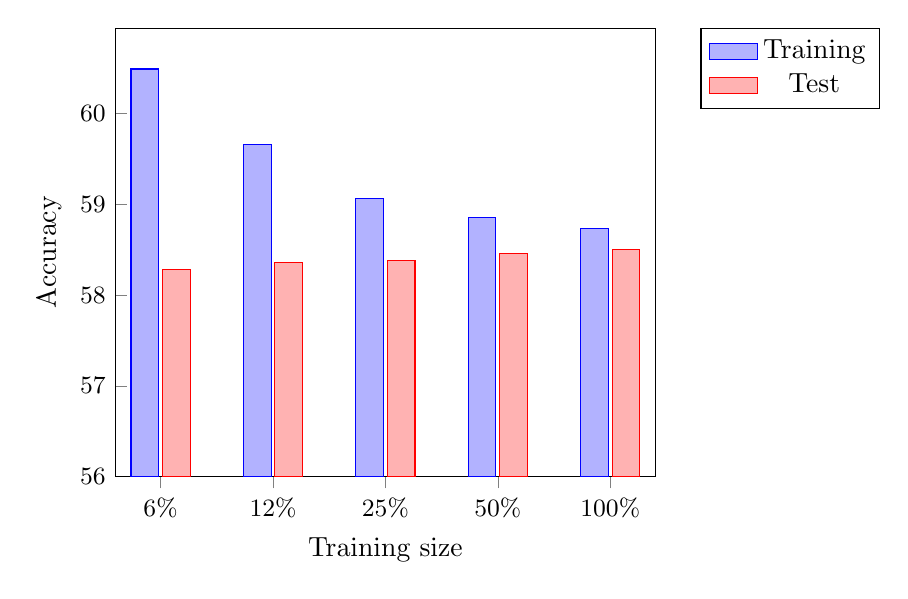
\begin{tikzpicture}
\begin{axis}[
    ybar,
    ylabel = Accuracy,
    xlabel = Training size,
    tick label style={font=\small},
    tickpos=left,
    xticklabels={6\%, 12\%, 25\%, 50\%, 100\%}, 
    xtick={1,2,3,4,5, 6},
    ymin=56,
    legend entries={Training,Test},
    legend style={at={(1.25,1.0)},
        anchor=north,legend columns=1
    },
    legend image code/.code={%
      \draw[#1] (0cm,-0.1cm) rectangle (0.6cm,0.1cm);
    }   
    ]   
    \addplot +[bar shift=-.2cm] coordinates {(1,60.49) (2,59.66) (3,59.06)  (4,58.85)     (5,58.73)  };

    \addplot  +[bar shift=.2cm]coordinates {(1,58.28) (2,58.36) (3,58.38) (4,  58.46) (5,58.50) };

\end{axis}
\end{tikzpicture}
  \caption{Experiment for representation of features}\label{fig:clusterbigdata}
\end{figure}

The results also shows that as the size of the training data increases overfitting decreases. The difference in accuracy between the training set and the test-set moves from $3.79\%$ for 84,529 matches to $3.79\times10^{-1} \%$ for 1,348,428 matches. We can also see that the model does not improve by much as the amount of data increases. The experiment shows that as the amount of data used for training increases, overfitting decreases severely. \todo{konklusion mangler}
% 0-vægte 
% 6: 71861
% 12: 65189
% 25: 60376
% 50: 56992
% 100: 54702

% total: 189183      


\subsubsection{Feature experiments}\label{sec:feattest}
A number of experiments are performed to see if combining different types of features may be beneficial.
Experiments are performed using logistic regression using stochastic gradient descent and L2 regularisation with a ridge value of 0.01. The different types of features used are:
\begin{enumerate}
\item $\phi_\text{SINGLE}$
\item $\phi_\text{PAIR}$
\item $\phi_\text{SINGLE}$, $\phi_\text{PAIR}$
\item $\phi_\text{SINGLE}$, $\phi_\text{PAIR}$, $\phi_\text{COUNTER}$
\item $\phi_\text{SINGLE}$, $\phi_\text{PAIR}$, $\phi_\text{COUNTER}$, $\phi_\text{BEST-RANK}$
\item $\phi_\text{all}$
\end{enumerate}

\begin{figure}[!htb]
  \centering
  % Graph for feature tests. 
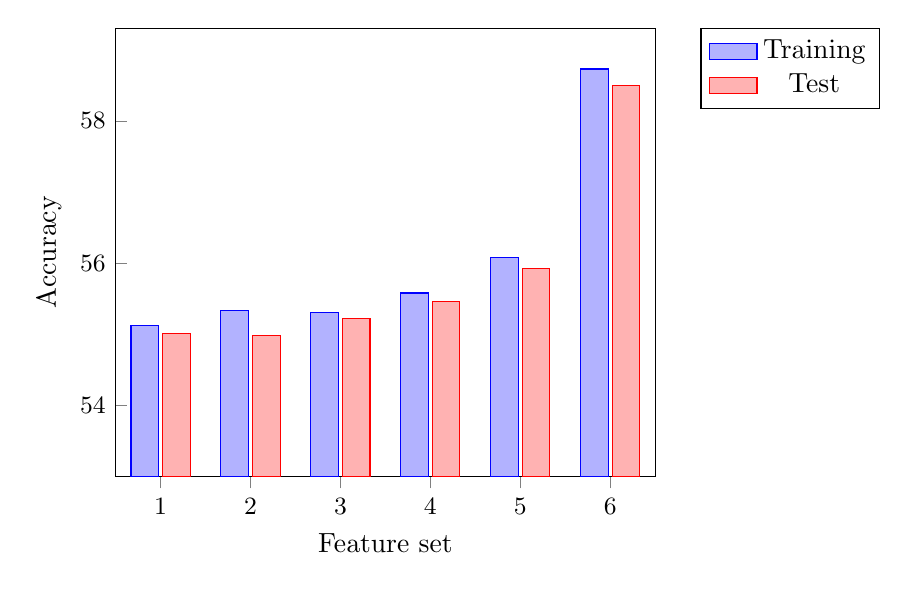
\begin{tikzpicture}
\begin{axis}[
    ybar,
    ylabel = Accuracy,
    xlabel = Feature set,
    tick label style={font=\small},
    tickpos=left,
    xticklabels={1, 2, 3, 4, 5, 6}, 
    xtick={1,2,3,4,5, 6},
    ymin=53,
    legend entries={Training,Test},
    legend style={at={(1.25,1.0)},
        anchor=north,legend columns=1
    },
    legend image code/.code={%
      \draw[#1] (0cm,-0.1cm) rectangle (0.6cm,0.1cm);
    }   
    ]   
    \addplot +[bar shift=-.2cm] coordinates {(1,55.12) (2,55.34) (3,55.31)  (4,55.58)     (5,56.08) (6, 58.73)};

    \addplot  +[bar shift=.2cm]coordinates {(1,55.01) (2,54.98) (3,55.22) (4,  55.46) (5,55.92) (6, 58.50)};

\end{axis}
\end{tikzpicture}
   \caption{Accuracy of feature sets. The features used for each test are shown in \Cref{sec:feattest}}\label{fig:cluster-feat}
\end{figure}

The feature evaluation results from \Cref{fig:cluster-feat} shows two interesting results, by looking at each individual case we can see that there is almost no overfitting. The largest difference is data point 2: (pairs) with a difference of $3.610^{-3}$ percentage points. The results shows some tendency between the complexity of the model and the performance of the classifier. Higher complexity in general yields a better classifier. The best result 58.5\% was achieved using all pre-match features.

%%% Local Variables:
%%% mode: latex
%%% TeX-master: "../main"
%%% End:
